\documentclass[final]{article}

\usepackage{nips_2017}
\usepackage[utf8]{inputenc} % allow utf-8 input
\usepackage[T1]{fontenc}    % use 8-bit T1 fonts
\usepackage{hyperref}       % hyperlinks
\usepackage{url}            % simple URL typesetting
\usepackage{booktabs}       % professional-quality tables
\usepackage{amsfonts}       % blackboard math symbols
\usepackage{graphicx}
\usepackage{xcolor}
\usepackage{float}

\title{SMPL-Based Motion Dataset Explorer and Generator}


\author{
  Vijay~Kotta and Faheem~Khawar\\
  Group \#: 9 \\
  Department of Computer Science, Department of Economics\\
  % Department of \(Computer Science\)\\
  University at Buffalo\\
  Buffalo, NY 142603 \\
  \texttt{\{vkotta;faheemkh\}@buffalo.edu} \\
}

\begin{document}

\maketitle

\begin{abstract}

This paper investigates the robustness of the Skinned Multi-Person Linear (SMPL) model, a state-of-the-art parametric body model that represents human body shape and pose through learned blend shapes and joint rotations. SMPL captures realistic body shape variation and pose-dependent deformations that prior models could not adequately represent. We introduce controlled Gaussian perturbations and noise to the model's shape and pose parameters and examine how these disturbances affect the quality of the reconstructed body mesh, evaluating the model's sensitivity to noise across varying magnitudes. The SMPL model and its pretrained parameters are obtained from the official release (version 1.0.0, 10 shape principal components).

  % The abstract must be limited to one paragraph and should summarize the entire document, briefly stating your problem definition, your methodology, the nature of the dataset tested on and lastly how you evaluated your methodology. Should be no more than 300 lines.
\end{abstract}

{\section{Introduction}}\label{sec:intro}
Describe the problem you are solving and explain its relevance to society in general. Why should anyone care about this problem? Next briefly explain the merits of your proposed approach. Why are you approaching the problem in this manner and not using some other known strategies? \\

\section{Related works}\label{sec:past}

An influential paper on this project is \textit{Self-supervised 3D Human Mesh Recovery from Noisy Point Clouds} by Zuo et al. \cite{ZuoWSGC21} The paper focused on using a Gaussian Mixed Model to model the point cloud as the input, as opposed to manually predicting the correspondences of each vertices in a point cloud. The former method is much more tolerant to outliers, while the latter struggles. Additionally, using a GMM works well even for incomplete point clouds, while the other way is forced to need complete point clouds. This fact is one that has caused many problems in other models at the time, as the data used for them have been far too “clean” than is realistic.

More importantly for our paper, it was found that using a GMM is quite robust even when Gaussian noise and random outliers were added to the data with only small changes in performance. Increasing $\sigma^2$, on the other hand, did lead to modest changes as large values force the network to poorly fit the inputs. Overall, this paper raises important points on how changing the variation and distinctness of the inputs, sometimes to match what they may look like in real life, can affect model performance.

Another helpful paper was \textit{Robust Human Registration with Body Part Segmentation on Noisy Point Clouds} by Lascheit et al. \cite{LascheitBPGE25}. Their contribution is using a hybrid approach which first looks at individual points and assign body part labels, then use a SMPL-X fit of the initial pose and orientation using said body parts, finally ending with global refinement (of the point cloud).

Their methods are tested with datasets which have some sort of difficult feature to them, such as partial observations or occlusions. Their results show great performance of such datasets compared to the other models at the time. The key takeaway from this paper for this project is that assigning body part labels can massively assist in the model predicting and modeling well of data that inherently has high variation. Along the lines of noise, the dataset consisted of many difficult features which forced the model to adapt and predict in ways that may mirror realistic inputs more precisely.

In \textit{SMPL Variable Model for 3D Reconstruction and Image Fusion in Animation Media Applications} \cite{XieZ25}, the authors proposes a novel deep learning network mode of animation, AniReconstructNet has created three new architectural avenues to expand upon the existing SMPL model: (1) a soft tissue layer of variable thickness that allows the representation of anatomically non-uniform deformations, (2) a UV mapping system which allows the 3D mesh to be projected into a 2-dimensional coordinate system of fixed resolution for the purpose of inferring the deformation through a convolutional neural network (CNN) and (3) a force conditioning mechanism which encodes both external forces and body pose into a shared latent vector to facilitate the deformation of the soft tissue. The final framework was tested using four different datasets (ShapeNet, ShapeNetCore, ABC, Scan2CAD) and exhibited improved performances in terms of accuracy, recall, F1 score, and AUC of from 2 to 4\%, as well as having fewer parameters, less FLOPs, lower inference times, and smaller memory consumption than any of the current leading deep learning methods.

This paper is directly relevant to any SMPL extension that aims to model phenomena beyond the original model's scope, particularly soft tissue dynamics and interaction. The variable thickness soft tissue layer concept addresses one of SMPL's explicitly acknowledged limitations: that poses dependent blend shapes are body shape independent. Extending this idea to make deformation stiffness a function of body composition such as BMI, fat distribution could be a meaningful direction. The UV-space deformation strategy is also a practically important technique, since it enables CNN-based processing of mesh deformations without requiring graph based or point cloud architectures. The force conditioning mechanism, while underdeveloped in the paper, suggests a promising avenue for modeling human environment interactions, which SMPL based reconstructions typically ignore. I could adopt a more rigorous version of this force modeling grounded in physical simulation rather than the purely learned approximation used here.

Furthermore, in \textit{SMPL-A: Modeling Person-Specific Deformable Anatomy} \cite{GuoPZKCW22}, the authors presented SMPL-A, which is the first learning based framework that enhances the standard SMPL with an estimate of internal organ deformity conditioned on patient pose. Whereas all the SMPL models have been developed to characterize the external surface of the human body, SMPL-A adds a new parameter ($\alpha$). Parameter $\alpha$ encodes patient specific shape and elastic properties of the patient's internal organs (lungs, liver, spleen, kidneys) when the patient is in a specific pose. By using past medical scans of the patient and the current pose of the patient, SMPL-A can estimate how the patient's internal organs have deformed as a function of changes in body pose. This will directly help with clinical applications such as planning for radiotherapy and surgery because it is critical to accurately locate the person's organs intra-operatively without exposing them to radiation multiple times.

Of the three pieces we surveyed here, this one is probably most ambitious from an intellectual standpoint, it also presents a type of SMPL extension that is largely unrelated to what was introduced at the outset of the original paper's focus. SMPL-A provides an important avenue for research on the coupling of the external human body model (as captured in SMPL) to the internal anatomical structure of the body. Although your application may be di[erent (e.g., contained within areas such as animation and/or pose estimation), the conceptual model presented in SMPL-A (i.e., a low-dimensional latent parameter that allows additional structure to be added but is disassociated from both pose and shape) can also be used in the application of your extension. This means that you can use the encoder decoder model in SMPL-A with $\alpha$ representing the variable, i.e., the person factored into the model. In addition, the FEM augmented data generation methodology can be applied to any instance where the ground-truth deformation information is sparse and is thus commonly considered to be a significant roadblock to various SMPL extension projects.

Finally, in \textit{3D Human Body Reconstruction Based on SMPL Model} \cite{ChenSLMZJ22}, the authors present an optimization based framework for reconstructing the SMPL model from a single monocular image. The central innovation is a \textit{multi-term objective function} that jointly minimizes four loss components: 2D joint reprojection error ($E\{J, 2D\}$), 3D joint coordinate error ($E\{J, 3D\}$), \textbf{facial landmark alignment error} ($E_F$), and body prior regularization ($E_P$). The 3D joint loss addresses the depth ambiguity inherent to 2D projection to 3D projection, while the facial landmark loss constrains the head orientation, a degree of freedom that standard SMPL joints cannot uniquely determine since SMPL has only a single chin joint. HMR regression estimates are used to initialize parameters, accelerating convergence and avoiding local minima. Experiments on MPI\_INF\_3DHP, 3DPW, and LSP datasets demonstrate improved MPJPE and PA-MPJPE scores over SMPLify and HMR baselines.

While this paper does not extend SMPL's model architecture, but it is directly related to my project that needs to fit the SMPL model to real images or video. In my extension I will be introducing new Gaussian disturbances to the parameter as like in this paper my extension may also include introducing new model parameters such as SMPL-A introduces $\alpha$ \cite{GuoPZKCW22}, or as SMPL-X introduces hand and face parameters, the multi-term optimization framework described here provides a template for how to design fitting objectives that are both robust and well-conditioned. In particular, the facial landmark term demonstrates that auxiliary geometric signals from 2D detectors, even imperfect ones, can substantially constrain under determined degrees of freedom in the body model.

% Give an overview of what has been done already in the field have done relating to this problem either using similar datasets or similar approaches? Your literature review should synthesize, not merely summarize, prior work on diffusion models (or some other approach if you are not working with diffusion) relevant to your project. Organize the literature by technical themes, explain the core diffusion formulation needed to understand the reviewed methods, compare representative papers using common criteria, and discuss their evaluation protocols. 

%  Here are examples of using citations in latex \cite{deceptionCues03}. Then the second \cite{EnosBCGHS06} and the third \cite{GraciarenaSSEHK06}. 
 
%  Conclude by positioning your project within an open gap in the literature


\section{Data}

\subsection{Data}

The SMPL model is defined by a set of learned weights derived from thousands of 3D body scans collected by the Max Planck Institute for Intelligent Systems~\cite{SMPL:2015}. These scans capture a wide range of human body shapes and poses, and from them the authors extracted a statistical model through principal component analysis (PCA) and pose-dependent blend shapes. The result is a compact set of parameters that enables any user to generate a realistic 3D mesh of the human body by specifying a shape vector $\beta \in \mathbb{R}^{10}$ and a pose vector $\theta \in \mathbb{R}^{72}$.

This project uses the SMPL version 1.0.0 model files, available for download from the official project website.\footnote{\url{https://smpl.is.tue.mpg.de/download.php}} The download provides two \texttt{.pkl} files corresponding to the male and female body models respectively. Each file contains variables such as blend weights, the joint regressors, template shape, and the linear blend skinning weights. The shape space is defined by 10 shape principal components (PCs), which are the basis vectors that explain the greatest variance in body shape across the original dataset of 3D body scans. Adjusting the coefficients of these PCs controls attributes such as height, weight, and limb proportions.

Because the SMPL parameters are pretrained and distributed as a complete model, no additional data collection, annotation, or preprocessing was required for this project. The input to our experiments is the model itself: we systematically perturb the shape ($\beta$) and pose ($\theta$) parameters with controlled Gaussian noise at varying levels and observe the resulting changes in the output. This means our evaluation does not rely on external labeled datasets but instead by comparing the results from the altered parameters to that of the original parameters.

% In this section, provide a detailed description of the data you worked on. What type of data is it?  How or where did you get the data? How much will you have access to and will you be able to successfully evaluate your work with it (i.e.~the types of labels/annotations that exist on the dataset)? Did you have to do any preprocessing, filtering, or other special treatment to use this data in your project? If this is from another project or paper, include appropriate references. If you are downloading it, say from \emph{github}, add a link to the location of the data on-line and a brief description of what its original use. 

% It is helpful include sample images to help your reader better understand the type of data you are presenting/explaining.

\subsection{Visual data}
This is just a demonstration of incorporating multiple images within one structure to show how to use tabular columns within graphics environment.
\begin{figure}[H]
	%\vspace*{-7mm}
	\centering
	\begin{tabular}{cc}
		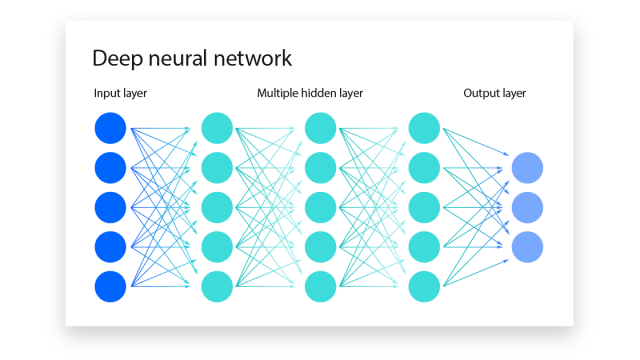
\includegraphics[width=0.5\linewidth]{image1} &
		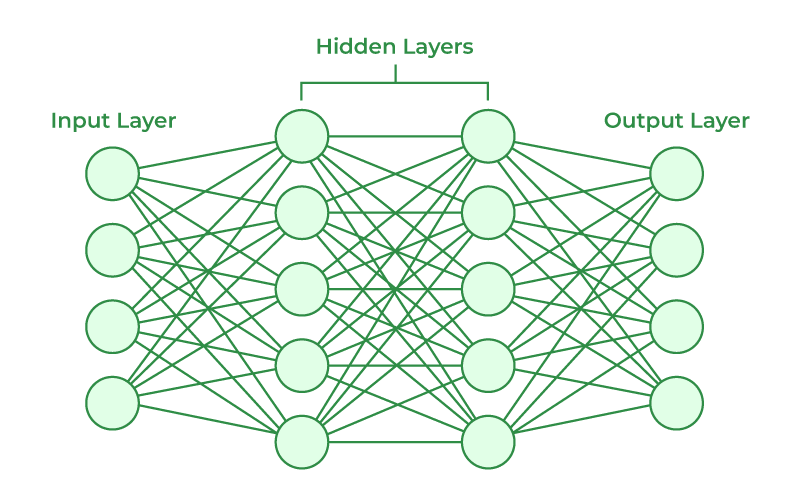
\includegraphics[width=0.5\linewidth]{image2} \\
		(a) Image 1: colored network &
		(b) Image 2: monochrome network \\
	\end{tabular}
	\caption{Two neural network diagrams colored differently}\label{img:2nns}
\end{figure}

\subsection{Audio data}
This is another subsection but here we introduce how to use tables such as in Table \ref{tab:table1} below. This is very common in the evaluation or results sections.
%
\begin{table}[H]
\centering
\caption{An example of a table reporting results.}\label{tab:table1}
	\begin{tabular}{|cccccc|}
		\hline
		Group & One     & Two     & Three    & Four     & Sum      \\ \hline\hline
		Red   & 1000.00 & 2000.00 &  3000.00 &  4000.00 & 10000.00 \\ \hline
		Green & 2000.00 & 3000.00 &  4000.00 &  5000.00 & 14000.00 \\ \hline
		Blue  & 3000.00 & 4000.00 &  5000.00 &  6000.00 & 18000.00 \\ \hline\hline
		Sum   & 6000.00 & 9000.00 & 12000.00 & 15000.00 & 42000.00 \\ \hline\hline
	\end{tabular}
\end{table}


\section{Methods}\label{sec:approach}
Discuss your approach for solving the problem that you set up in the introduction. Why is your approach the right thing to do? Did you consider alternative approaches? You should demonstrate that you have applied ideas and skills built up during the semester to tackling your problem of choice. It may be helpful to include figures, diagrams, or tables to describe your method or compare it with other methods.

\subsection{Innovation}
This is a critical piece of the report since it describes any changes or extensions you were able to make. It could be an extension to the Method, additional data that you collected and ran the model on, a new type of evaluation you performed on the model, etc. It's find if no additional tweaks were made; simply state it here.


\section{Experiments and Results}\label{sec:expts}
Discuss the experiments that performed to demonstrate that the approach solves the problem.  Exact experiments will vary depending on the project, but you might compare with previously published methods, perform an ablation study to determine the impact of various components of the system, experiment with different hyperparameters or architectural choices, use visualization techniques to gain insight into how your model works, discuss common failure modes of your model, etc. Describe any evaluation methods used here including different metrics that you use to confirm that your technique really does work well. Present any numbers, tables or graphs here, to illustrate your experimental results.

\begin{figure}[H]
	\centering
	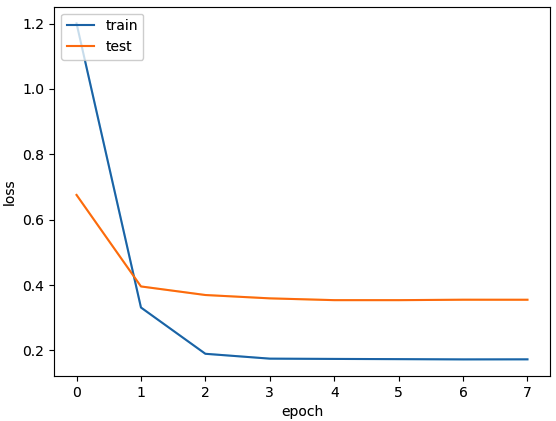
\includegraphics[width=0.5\linewidth]{learning}
	\caption{Sample figure showing the training and validation errors from a learning system.}
	\label{fig:aus}
\end{figure}

\section{Project limitations}\label{sec:limits}
State the limitations of your process and approach and explain why things did not work as well or why they worked so well. Also, explain why your work might or might not generalize to other datasets. This piece is not graded. It's just informational for the Instructors and TAs.

\section{Conclusion and future work}\label{sec:concl}
Summarize the key results you observed - what have you learned? What are your conclusions from the entire process; what did you leave undone and why? If someone else was going to pick up where you left off, what will be the most important aspects they should focus on? In general, suggest ideas for future extensions or new applications of your idea.  \medskip

\section{Contributions}

\small
%Your references will be automatically populated here as long as you enter them correctly into your .bib file. An example is attached
\bibliographystyle{plainnat}
\bibliography{references}

\end{document}











